\section{APU}
\label{sec:pp-apu}

Zvukový procesor APU (\textit{Audio Processing Unit}) není samostatným čipem, ale je integrován
přímo do CPU. Jeho registry jsou mapovány do adresového prostoru CPU v~rozsahu
\texttt{\$4000–\$4013}, \texttt{\$4015} a~\texttt{\$4017}; naprostá většina z~nich je pouze pro
zápis. APU disponuje pěti zvukovými kanály: dvěma generátory pulzního signálu (Pulse 1, Pulse 2),
generátorem trojúhelníkové vlny (Triangle), generátorem šumu (Noise) a~kanálem delta modulace pro
přehrávání vzorků (DMC).

\begin{figure}[H]
    \centering
    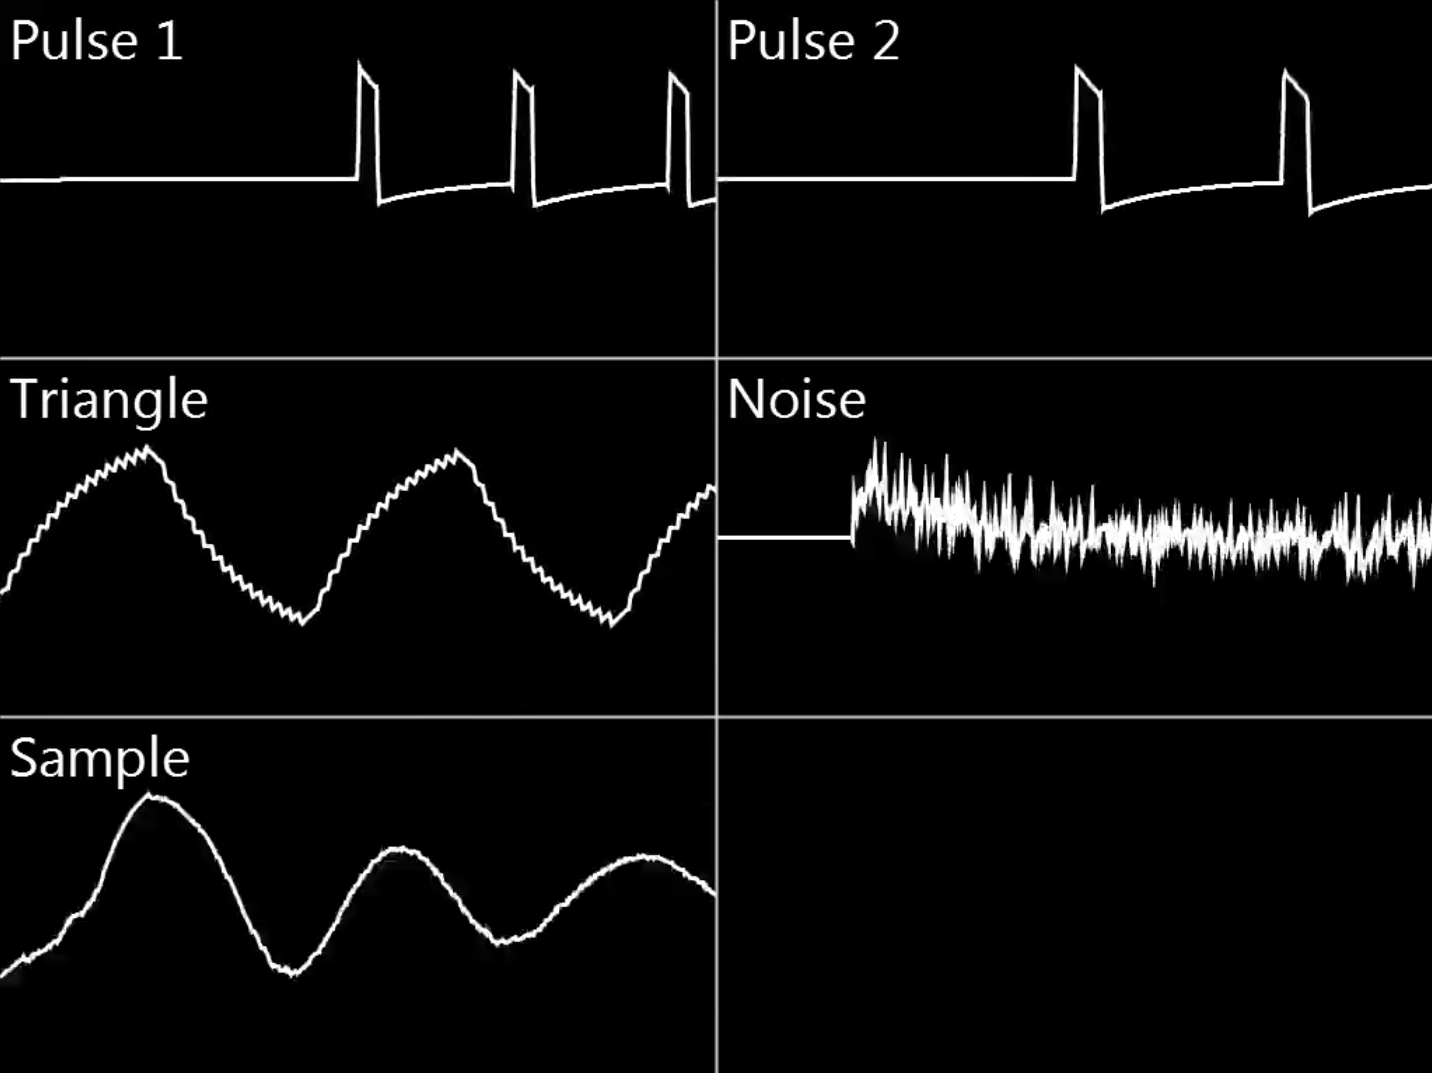
\includegraphics[width=0.5\textwidth]{images/apu_channels.png}
    \caption{Přehled zvukových kanálů APU. Zdroj \cite{copetti-nes}.}
    \label{fig:apu_channels}
\end{figure}

\subsection{Časování}

Taktová frekvence APU je přibližně stejná jako u CPU. Většina zvukových kanálů však jsou taktovány
poloviční frekvenci nebo i menší; jejich komponenty jsou místo toho řízeny hierarchií děličů
(\textbf{dividerů}) a~\textbf{timerů}, které z~tohoto základního taktu odvozují potřebné frekvence.

Klíčovým pojmem je \textbf{perioda} (\textit{period}) -- udává, kolik APU cyklů musí uplynout, než
daná komponenta provede svůj krok. Konkrétní implementační mechanismus se nazývá divider -- sestupný
čítač, který se dekrementuje každý APU cyklus. Jakmile dosáhne nuly, vyvolá příslušnou akci a~je
znovu nastaven na hodnotu periody:

$$
\text{divider} = \text{period} \implies \text{čekej } period \text{ cyklů, pak proveď akci}
$$

V~hardwaru NES se divider realizuje dvěma způsoby. Pulzní a~trojúhelníkový kanál používají lineární
sestupné čítače. Kanál šumu, DMC a~snímkovací čítač jsou implementovány prostřednictvím lineárních
zpětnovazebních posuvných registrů (LFSR — \textit{Linear Feedback Shift Register}).

\textit{Timer} je terminologicky totožný s~dividerem — jedná se o~jiný název pro stejný mechanismus.
V~kontextu APU se slovem \textit{timer} zpravidla označuje divider řídící výšku tónu (pitch) kanálu,
zatímco ostatní dividery (pro obálku, sweep, délkový čítač) si ponechávají vlastní pojmenování. Toto
rozlišení je čistě konvenční.

\subsection{Struktura kanálů}

Každý zvukový kanál se skládá z~kombinace následujících funkčních podjednotek; konkrétní sada závisí
na typu kanálu:

\begin{itemize}
    \item \textbf{Timer} -- divider odvozující výstupní frekvenci kanálu. Hodnota jeho periody je
        zapisována CPU do příslušných registrů a~přímo určuje výšku tónu. Kanál je hardwarově
        ztišen, pokud perioda klesne pod minimální prahovou hodnotu.
    \item \textbf{Sekvencer} -- komponenta procházející pevně danou sekvencí hodnot a~předávající
        aktuální krok na výstup kanálu. Je řízen timerem; každým jeho tickem přejde na další pozici
        v~sekvenci. Sekvencer definuje tvar výstupní vlny — například 8krokovou sekvenci střidy
        u~pulzního kanálu nebo 32krokový trojúhelníkový průběh.
    \item \textbf{Envelope} -- generátor obálky řídící okamžitou hlasitost kanálu. Interně jde
        o~divider taktovaný snímkovacím čítačem; po každém svém ticku dekrementuje 4bitový čítač
        hlasitosti nebo jej (v~režimu smyčky) restartuje od maxima. Výsledná hlasitost může být
        odvozena z~tohoto čítače, nebo nastavena konstantně.
    \item \textbf{Sweep} -- jednotka automatického přelaďování dostupná pouze u~pulzních kanálů. Je
        to divider řízený snímkovacím čítačem, který periodicky upravuje hodnotu timeru (a~tedy
        výšku tónu) o~přírůstek daný bitovým posunem. Při překročení rozsahu je kanál automaticky
        ztišen.
    \item \textbf{Length Counter} -- čítač délky tónu přítomný ve všech kanálech kromě DMC. Umožňuje
        automatické ztišení kanálu po uplynutí přednastavené doby bez zásahu CPU. Hodnota délky se
        načítá z~pevné vyhledávací tabulky a~je taktována snímkovacím čítačem.
    \item \textbf{Linear Counter} -- dodatečný čítač délky specifický pro trojúhelníkový kanál.
        Oproti length counteru nabízí jemnější rozlišení (7bitová hodnota zadávaná přímo) a~je
        taktován dvakrát tak rychle.
\end{itemize}

\subsection{Snímkovací čítač (Frame Counter)}

Snímkovací čítač (\textit{frame sequencer}) je centrální řídicí jednotka APU taktující všechny
nízkofrekvenční komponenty -- envelope generátory, sweep jednotky a~délkové čítače. Navzdory svému
názvu nemá přímou vazbu na obrazový signál PPU; pojmenování odráží přibližnou shodu jeho výstupní
frekvence s~obnovovací frekvencí obrazu.

Sekvencer je sám vícekrokový divider: při každém svém ticku aktivuje různé podmnožiny komponent.
Konfiguruje se zápisem do registru \texttt{\$4017} do dvou režimů:

\begin{itemize}
    \item \textbf{4krokový režim} -- envelope a~linear counter jsou taktovány každý krok (přibližně
        240~Hz pro NTSC), sweep jednotky každý druhý krok (přibližně 120~Hz). Na konci čtvrtého
        kroku může volitelně generovat přerušení IRQ (\textit{frame IRQ}).
    \item \textbf{5krokový režim} -- přidáním pátého kroku se celkové tempo modulátorů snižuje
        (efektivní frekvence klesá na přibližně 48~Hz pro NTSC). Přerušení IRQ v~tomto režimu
        generováno není.
\end{itemize}

\subsection{Mixér a výstup}

Výstupy všech pěti kanálů jsou kombinovány interním mixérem se dvěma větvemi: pulzní větev (Pulse~1
+ Pulse~2) a~TND větev (Triangle + Noise + DMC). Každá větev má vlastní nelineární DAC, takže
výsledná amplituda není prostým součtem hodnot jednotlivých kanálů. Tato nelinearita způsobuje
vzájemné ovlivňování kanálů — například zápis do výstupního registru DMC (\texttt{\$4011}) mění
zdánlivou hlasitost trojúhelníkového a~šumového kanálu. Pro emulaci mixéru je možné použit
vyhledávací tabulku aproximovaných hodnot\cite{nesdev-apu-lut}:

\vspace{-0.75cm}

\begin{align*}
    % a = 5&&
    &\text{output} = \text{pulse}_{\text{out}} + \text{tnd}_{\text{out}}\\
    &\text{pulse}_\text{lut}[n] = \frac{95,52}{\frac{8128}{n} + 100}\\
    &\text{pulse}_\text{out} = \text{pulse}_\text{lut}[\text{pulse}_1 + \text{pulse}_2]\\
    &\text{tnd}_\text{lut}[n] = \frac{163,67}{\frac{24329}{n + 100}}\\
    &\text{tnd}_\text{out} = \text{tnd}_\text{lut}[3 \cdot \text{triangle} + 2 \cdot \text{noise} +
    \text{dmc}]
    % a
\end{align*}
